\newdateformat{mydate}{\monthname[\THEMONTH] \THEYEAR} 

\begin{titlepage}

	\newgeometry{left=30mm,right=-25mm,top=32mm,bottom=25mm}  
    
    % Kopfzeile
	\begin{table}[h!]
		\begin{tabular}{rp{5cm}l}
 		
\includegraphics[height=1.25cm]{../Logos/Cosima18.png} & & 
\includegraphics[height=1.25cm]{../Logos/TOS.png} \\
		\end{tabular}
	\end{table}
    
    \small
	\parindent0pt
	
	\begin{center}
		\bfseries Projektmappe für den COSIMA-Wettbewerb 2018
	\end{center}
	
	\vspace*{15mm}
	\normalsize	
	
	\begin{center}
		\huge
		{\bfseries\sffamily Der Gestikulaser}
		\\ \vspace*{4mm}
		\large
		Die neue Technologie der Gestenerkennung
	\end{center}
	
	\vfill
	
	\begin{center}
	\large \mydate{\today}
	\end{center}
	
	\centering
	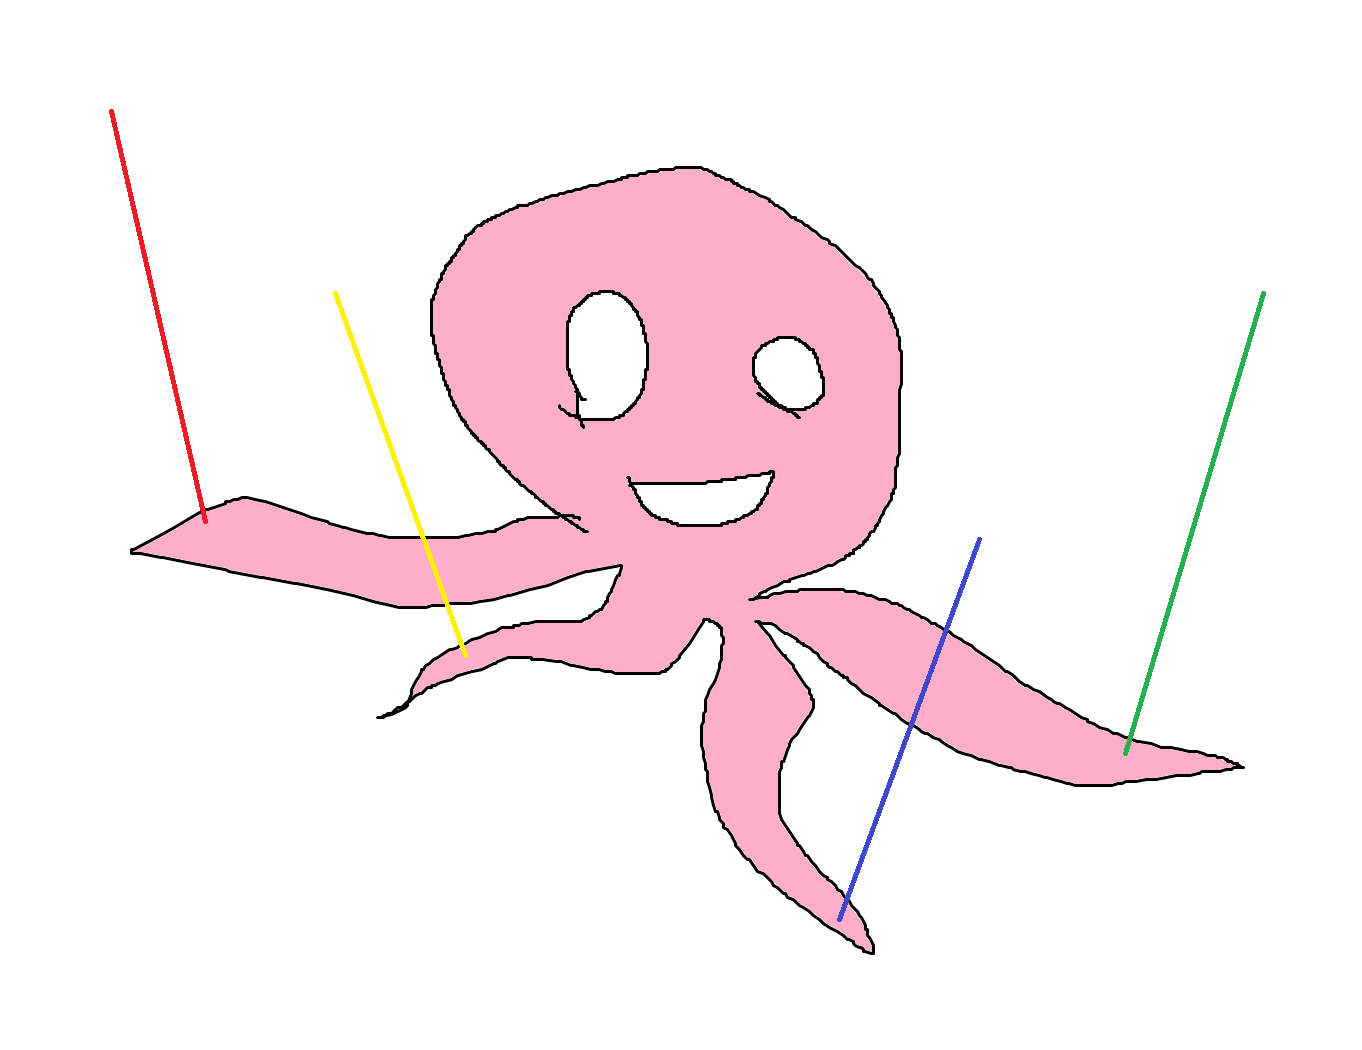
\includegraphics[width=15cm,height=9cm]{../figures/GestikulaserLogo.png}
	\vfill
	
	\begin{center}
		Verfasst von \\[3ex]
		Christoph Behr \\
		Cailing Fu \\
		Nicole Grubert \\
		Daniel Wolff \\
	\end{center}
	
	\restoregeometry
	
\end{titlepage}